% Disclaimer page
\begin{titlepage}
{\Large Welcome to the or-tools user's manual!}\\

\vspace{\stretch{1}}

\copyright\ Copyright 2012, Google\\


\vspace{\stretch{1}}

\section*{License information}

\fancyfoot{}
\fancyhead[LE,RO]{\textsc{\thepage}}

This document is provided under the terms of the 
\begin{center}
  \begin{large}\code{Apache License 2.0}\end{large}
\end{center}
You can find the complete license text at the following address: \url{http://www.apache.org/licenses/LICENSE-2.0}.\\

We kindly ask you not to make this document available on the Internet. This document should only be available at the following address:
\begin{center}
  \url{http://or-tools.googlecode.com/svn/trunk/documentation/documentation_hub.html}
\end{center}
This is the address of our documentation hub where you can find other useful sources of documentation about the \code{or-tools} library.

\section*{Trademarks}
GOOGLE is a trademark of Google Inc.\\
Linux is a registered trademark of Linus Torvald in the United States, other countries, or both.\\
Java and all Java-based trademarks and logos are trademarks of Sun Microsystem Inc. in the United States, or both.\\
Other companies, products, or service names may be trademarks or service marks of others.

\section*{Ackowledgments}
We thank the following people for their helpful comments:\\
Dania El-Khechen, H\r{a}kan Kjellerstrand, Louis-Martin Rousseau
\end{titlepage}

\begin{titlepage}
%%%%%%%%%%%%%%%%%%%%%%%%%%%%%%%%%%%%%%%%%%%%%%%%%%%%%%%%%%%%%%%%%%%%%%%
%\newpage
%\thispagestyle{plain}
\pagestyle{fancy}
\chapter*{Foreword}

We are glad to welcome you to the {\bf or-tools user's manual}. In this foreword, we try
to answer most common questions a newcomer could have when discovering this manual or the library for the first time.\\

The {\bf or-tools}~library is a set of operations research tools developed at Google. 
If you have no idea what \emph{operations research}\footnote{If you are curious: \href{http://en.wikipedia.org/wiki/Operations_research}{Wikipedia article on Operations research}.} is, 
you still can use our library to solve common small problems with the help of our Constraint Programming (CP) solver. If you do know what~\emph{operations research} is and how difficult it is sometimes to find efficient, 
easy to use and open source code, we hope you will enjoy using our library. We have put a lot of efforts in order to make it user friendly and continue to improve it
on a daily basis. Furthermore, we encourage interactivity and are always open to suggestions. See the section~\emph{How to reach us?} below. If you have comments about this manual or the documentation in general, see the section~\emph{Do you have comments?}.

\section*{What is or-tools?}

The {\bf or-tools}~library is a set of {\bf o}perations {\bf r}esearch {\bf tools} written in C++ at Google.

The main tools are:
\begin{itemize}
  \item A Constraint Programming solver.
  \item A simple and unified interface to several linear programming and mixed
integer programming solvers (GLPK, CLP, CBC and SCIP).
  \item Knapsack algorithms.
  \item Graph algorithms (shortest paths, min cost flow, max flow, linear sum assignment).
\end{itemize}

\newpage
\pagestyle{plain}
In short, the \emph{or-tools}~library is:

\begin{itemize}
 \item {\bf Open source and free} Everything, including the examples, the implementations of the algorithms, the various 
       documentations\footnote{The source code and the scripts used to generate the documentation will be available soon.},  
       is licenced under the \code{Apache License 2.0} and is available for download. If you make substantial improvements to our code, 
       please share it with the whole community.
 \item {\bf Alive} The library is actively maintained and updates and improvements are made on an almost daily basis.
 \item {\bf Documented} OK, we just started to write the documentation but there are already numerous examples written in \code{C++}, \code{Python}, \code{Java} and \code{C\#}!
 \item {\bf Portable} Because it is made by Google, the code conforms strictly to the Google coding styles\footnote{See for instance~\href{http://google-styleguide.googlecode.com/svn/trunk/cppguide.xml}{http://google-styleguide.googlecode.com/svn/trunk/cppguide.xml} 
 for the Google C++ Style Guide.}. The code is known to compile on:
	\begin{itemize}
    \item gcc 4.4.x on ubuntu 10.04 and up (10.10, 11.04, 11.10 and 12.04).
    \item xcode >= 3.2.3 on Mac OS X Snow Leopard and Mac OS X Lion (gcc 4.2.1).
    \item Microsoft Visual Studio 10. 
	\end{itemize}
Both 32 bit and 64 bit architectures are supported, although the code is optimized to run in 64 bit mode.    
 \item {\bf Efficient} 
 \item {\bf Accessible} Everything is coded in C++ but is available through SWIG in Python, Java, and .NET (using Mono on non-Windows platforms). 
 \item {\bf User-friendly} We try to make our code as easy to use as possible (especially in \code{Python} and \code{C\#}). 
       Of course, there is a (small) learning curve to use our library but once you master several basic concepts, it is quite straightforward to code with the \emph{or-tools} library. 
 \item {\bf Tested} We use it internally at Google since a few years and the community of users is growing.
\end{itemize} 
    
\section*{What you will learn in this document}

This manual is intended to give you the necessary knowledge to use the library and explore the reference manual by yourself. We describe the basic concepts but also
how to customize your search in Constraint Programming (CP). One of the strength of our library is its \emph{routing} solver in CP to solve arc- and vehicle routing problems with constraints.
We describe how to customize your routing algorithms. After reading this manual, you will be able to understand our way of coding and how to use the
full potential of our library. 
    
\section*{What you will not learn in this document}

This document is by no means a tutorial on Operations Research nor on Contraint Programming. 
It is also NOT a reference manual (refer to the \href{http://or-tools.googlecode.com/svn/trunk/documentation/documentation_hub.html}{documentation hub} to find the \href{http://or-tools.googlecode.com/svn/trunk/documentation/reference_manual/or-tools/index.html}{reference manual}).
There are way too many methods, parameters, functions, etc. to explain them all in details. Once you understand the concepts and methods explained in this manual, you shouldn't have any trouble scanning the
\href{http://or-tools.googlecode.com/svn/trunk/documentation/reference_manual/or-tools/index.html}{reference manual} and find the right method, parameter, function, \ldots\ or code them yourselves!\\

We don't document the non Constraint Programming (CP) part of the library. If you have any questions about the non-CP part of the library, don't hesitate to ask
them on the mailing list. See the section~\emph{How to reach us?} below.\\

This document will not describe how to use the library (and the syntactic sugar introduced when possible) with \code{Python}, \code{Java} nor~\code{C\#}. This could possibly change in the future. The tutorial examples (see below) exist also in \code{Python}, \code{Java} and~\code{C\#} though. 

\section*{How to read this document?}

You could read this document from cover to cover but we have put a lot of efforts to make each chapter stands on its own.
The best way to read this manual is to look for a specific answer, use the index, the table of contents or the glossary to find a reference to that information.
If you are missing some requirements to understand a section, you can always backtrack on prerequisite knowledge. For each chapter, we list those prerequisites. This
non-linear way of reading is probably the most efficient and rewarding one!\\

That said, the manual is kept short so that you can read it in its entirety. The first part (\emph{Basics}) is an introduction on how to use the CP solver
to solve small problems. For real problems, you need to customize your search and this is explained in the second part (\emph{Customization}). If you are interested
in the routing part of the library, the third part is for you (\emph{Routing}). Finally, some utilities and tricks are explained in the last part (\emph{Technicalities}).

\section*{Targeted audience}

This manual is written with two types of readers in mind. First, someone who is not familiar with Constraint Programming
    nor is she a professional programmer. Second, an educated reader who masters Constraint Programming and is quite at ease without
    necessarily mastering one of the supported computer languages. Did we succeed to write for such different profiles? You tell  
    us! 
    
\section*{Conventions used in this manual}

All the code is systematically written in \code{monospace font}. Function and method's names are followed by parentheses. The method \code{MakeSomething()} and
the parameter \code{something} are two beautiful examples of this convention.\\

To draw your attention on important matters, we use a box with a danger warning sign.\\

\begin{notice}{warning}{Warning:}
You have been warned!
\end{notice}
~\\

To explain some details that would break the flow of the text, we use a shadowed box.

\setbox0\vbox{
\begin{minipage}{0.95\linewidth}
\textbf{This is an explanation that would break the flow of the text}

\medskip

This is why we prefer to put our explanation aside in a shadowed box.
\end{minipage}}
\begin{center}\setlength{\fboxsep}{5pt}\shadowbox{\box0}\end{center}

To focus on some parts of the code, we omit non necessary code or code lines and replace them by~"\ldots".

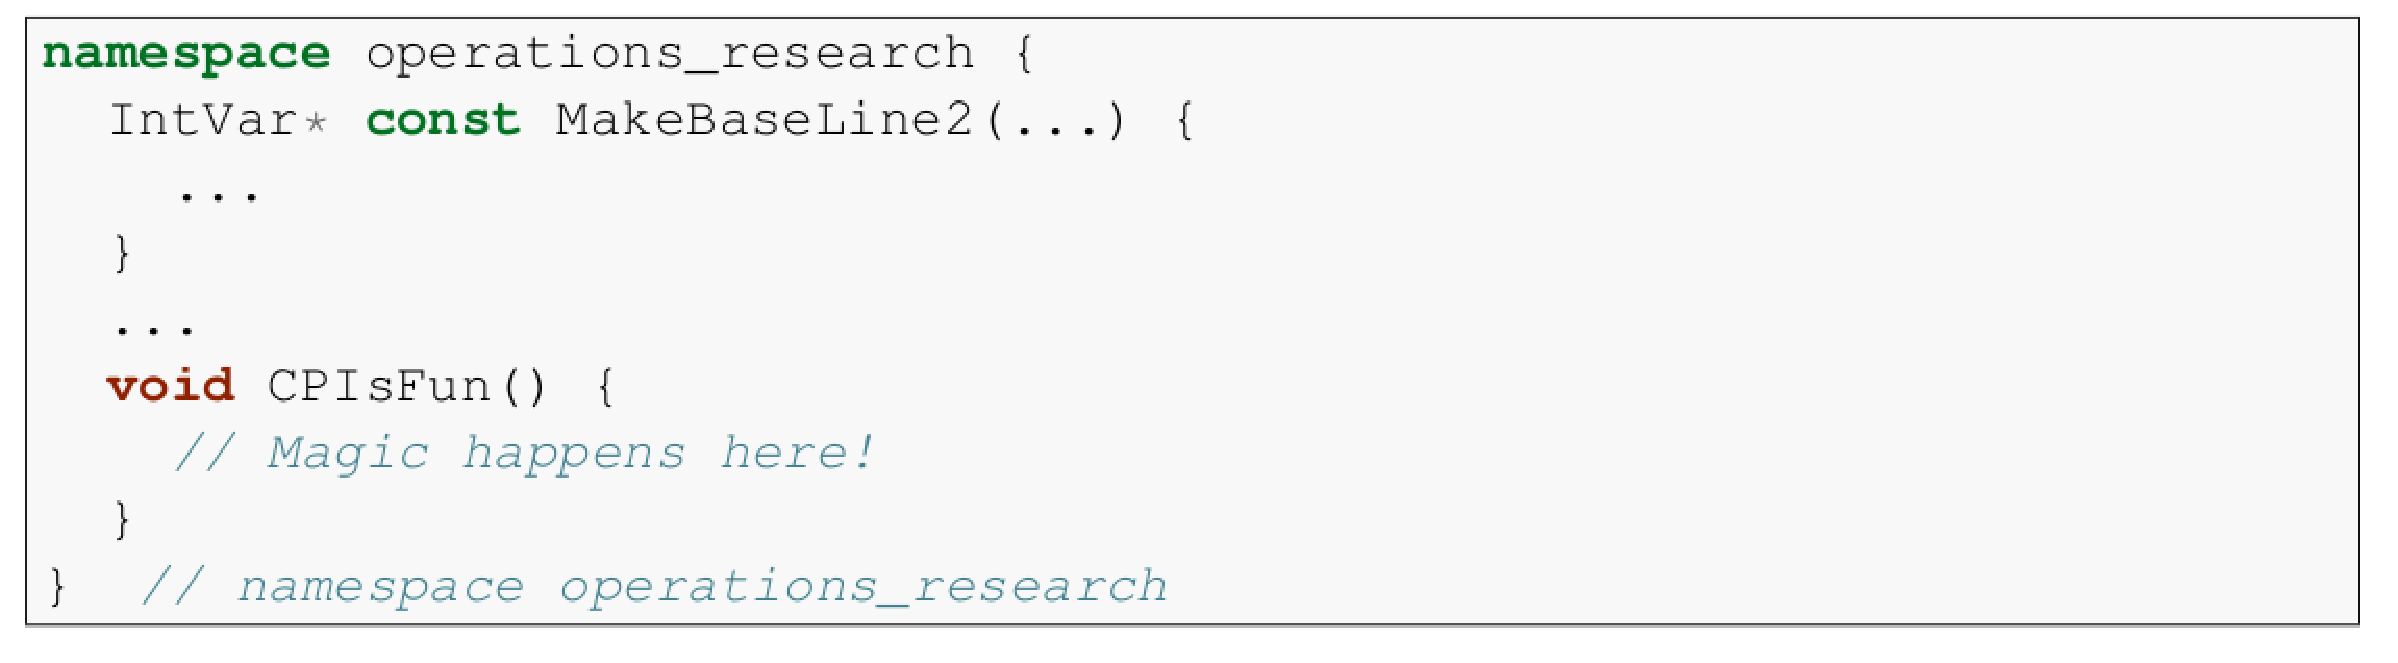
\includegraphics[width=1.05\linewidth]{code_example.pdf}
In this example, the parameters of the function~\code{MakeBaseLine2()} are stripped as are the content of this method and the code lines that follow the definition
of this function. The purpose of this example is to show that the code is written inside the~\code{namespace}~\code{operations\_research}.

All commands are issued from a Unix-like terminal:

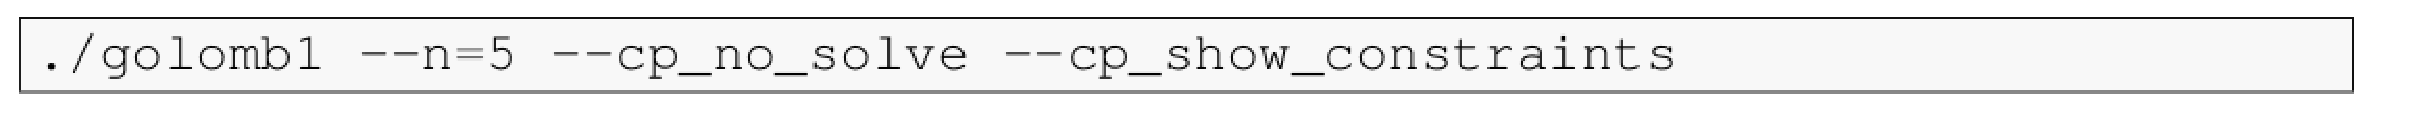
\includegraphics[width=1.06\linewidth]{command_line.pdf}
Adapt the command lines to your type of terminal and operating system.

\section*{Accompanying code for this manual}

All the examples in this manual are coded in \code{C++}. For the most important code snippets, you can find complete examples on the documentation hub:\\

\begin{center}
  \url{http://or-tools.googlecode.com/svn/trunk/documentation/documentation_hub.html\#tutorial_examples}
\end{center}

or under the following directory of the or-tools library:\\

\code{documentation/tutorials/C++}\\

If you prefer to code in \code{Python}, \code{Java} or \code{C\#}, we have translated all the examples in your favourite language. You can find the complete examples on the documentation hub or under the directories:\\

\code{documentation/tutorials/Python}\\
\code{documentation/tutorials/Java}\\
\code{documentation/tutorials/Csharp}.

\section*{Lab sessions}

Theory is good but useless without practice and experience. For each chapter, we provide exercises. Most of them are practical and consist in completing some~\code{C++} code. 
Even if you don't (like to) code in~\code{C++}, these lab sessions are helpful as we develop some concepts seen in the manual more in details. Exercises vary between simple and 
straightforward to sometimes really challenging. In the latter case, we mark these exercises as such. For all the exercises, we provide solutions.\\

You can find (soon!) the exercises and their solutions on the documentation hub:\\

\begin{center}
  \url{http://or-tools.googlecode.com/svn/trunk/documentation/documentation_hub.html\#lab_sessions}
\end{center}

or under the following directory of the or-tools library:\\

\code{documentation/labs/C++}

\section*{How to reach us?}
\label{how_to_reach_us}
The whole project \code{or-tools} is hosted on Google code:\\
\begin{center}
\url{http://code.google.com/p/or-tools/}\\
\end{center}

You can follow us on Google+:\\
\begin{center}
\url{https://plus.google.com/u/0/108010024297451468877/posts}
\end{center}
and post your questions, suggestions, remarks, \ldots\ to the~or-tools~discussion~group:
\begin{center}
\url{http://groups.google.com/group/or-tools-discuss}
\end{center}

\section*{How to reference this document?}

Use this simple reference:
\begin{center}
N. van Omme and L. Perron, \emph{or-tools user's manual}, Google, 2012.
\end{center}

Here is a bibtex entry:

\code{%
\symbol{64}TECHREPORT\{or-tools-user-manual,\\
\hspace*{5mm}  author = Nikolaj van Omme and Laurent Perron,\\
\hspace*{5mm}  title = or-tools user's manual,\\
\hspace*{5mm}  institution = Google,\\
\hspace*{5mm}  year = 2012\\
\}
}

\section*{Do you have comments?}

If you have comments, suggestions, corrections, feedback, \ldots,  about this document or about the documentation of the or-tools library in general, please send them
to \href{mailto:ortools.doc@gmail.com}{ortools.doc@gmail.com}. Thank you very much.


~\\
Happy reading!\\

The or-tools team
\end{titlepage}
